\documentclass[10pt,journal,compsoc]{IEEEtran}
\usepackage[utf8]{inputenc}

% *** CITATION PACKAGES ***
%
\ifCLASSOPTIONcompsoc
  % The IEEE Computer Society needs nocompress option
  % requires cite.sty v4.0 or later (November 2003)
  \usepackage[nocompress]{cite}
\else
  % normal IEEE
  \usepackage{cite}
\fi
\usepackage{graphicx}
\usepackage{caption}
\usepackage{eurosym} 
\renewcommand{\tablename}{Tab.}
\graphicspath{ {images/} }
% *** GRAPHICS RELATED PACKAGES ***
%
\ifCLASSINFOpdf
  
\else
 
\fi
\newcommand\MYhyperrefoptions{bookmarks=true,bookmarksnumbered=true,
pdfpagemode={UseOutlines},plainpages=false,pdfpagelabels=true,
colorlinks=true,linkcolor={black},citecolor={black},urlcolor={black},
pdftitle={Bare Demo of IEEEtran.cls for Computer Society Journals},%<!CHANGE!
pdfsubject={Typesetting},%<!CHANGE!
pdfauthor={Michael D. Shell},%<!CHANGE!
pdfkeywords={Computer Society, IEEEtran, journal, LaTeX, paper,
             template}}%<^!CHANGE!

\hyphenation{op-tical net-works semi-conduc-tor}


\begin{document}

\title{Sistema domótico IoT basado en Raspberry Pi y control remoto por Telegram}
\author{Jesús Gómez Bellido}

% for Computer Society papers, we must declare the abstract and index terms
% PRIOR to the title within the \IEEEtitleabstractindextext IEEEtran
% command as these need to go into the title area created by \maketitle.
% As a general rule, do not put math, special symbols or citations
% in the abstract or keywords.
\IEEEtitleabstractindextext{%
\begin{abstract}
The abstract goes here.
\end{abstract}

% Note that keywords are not normally used for peerreview papers.
\begin{IEEEkeywords}
Computer Society, IEEE, IEEEtran, journal, \LaTeX, paper, template.
\end{IEEEkeywords}}


\maketitle


% To allow for easy dual compilation without having to reenter the
% abstract/keywords data, the \IEEEtitleabstractindextext text will
% not be used in maketitle, but will appear (i.e., to be "transported")
% here as \IEEEdisplaynontitleabstractindextext when compsoc mode
% is not selected <OR> if conference mode is selected - because compsoc
% conference papers position the abstract like regular (non-compsoc)
% papers do!
\IEEEdisplaynontitleabstractindextext
% \IEEEdisplaynontitleabstractindextext has no effect when using
% compsoc under a non-conference mode.


% For peer review papers, you can put extra information on the cover
% page as needed:
% \ifCLASSOPTIONpeerreview
% \begin{center} \bfseries EDICS Category: 3-BBND \end{center}
% \fi
%
% For peerreview papers, this IEEEtran command inserts a page break and
% creates the second title. It will be ignored for other modes.
\IEEEpeerreviewmaketitle


\ifCLASSOPTIONcompsoc
\IEEEraisesectionheading{\section{Introduction}\label{sec:introduction}}
\else
\section{Introduccion y objetivos}
\label{sec:introduction}
\fi

\IEEEPARstart En este Trabajo fin de Máster (TFM) vamos a tratar de ver el impacto que pueden generar las nuevas tecnologías que se están empezando a expandir.
Estas nuevas tecnologías tienen siempre en mente una perspectiva, el llamado "Internet of Things" (IoT) o Internet de las Cosas. 
Este es un término se refiere a la interconexión de dispositivos físicos, vehículos, edificios y otros objectos --embebidos con electrónica, software, sensores, actuadores y conexión a internet que permiten la recolección de datos.
Todo esto nos permite que los ordenadores interactúen con elementos de la vida real y ganen independencia de los seres humanos.

Bien es cierto, que el IoT va a suponer un gran impacto en cuanto a la industria y la investigación, pero no será menos para los ambientes domésticos ya que nos permite automatizar muchas funciones de nuestros hogares.
En este entorno tiene gran parte de importancia el uso de los \textit{smartphones}, pues son en muchos casos los encargados de comunicar a los seres humanos con nuestros dispositivos.

Otro de los dispositivos en auge y que han fomentado la automatización en los hogares son los micro-ordenadores, como son las Raspberry Pi, estos son dispositivos tremendamente versátiles y cada vez más potentes.


\subsection{Objetivos}
En el actual TFM, vamos buscar unos objetivos basándonos en IoT en un entorno doméstico.
Se realizará un sistema domótico básandonos en los principios del IoT.

Para llevar a cabo el primer objetivo, se va a usar una Raspberry Pi programandose con NodeJS, un entorno de ejecución para JavaScript, y viendo las posibilidades que este lenguaje nos proporciona en relación a Python, el cuál se puede decir que es el lenguaje de programación estándar para la Raspberry Pi.

El sistema domótico, realizará el control sobre persianas/toldos, basándose en las previsiones de servicios meteorológicos, prevaleciendo las acciones del usuario. El usuario también tendrá control sobre puertas, luces, el sistema de climatización y la alarma.

Por otro lado también se tendrá un control de presencia dentro de la casa, registrando las entradas y salidas de los usuarios mediante la MAC de su smartphone y el protocolo ARP. 

Por último, el control de nuestro sistema domótico se realizará mediante Telegram, las aplicaciones de mensajerías son algo indispensable hoy en día para las personas, así que viendo la API que este servicio de mensajería nos proporciona para realizar bots, parece interesante estudiar qué clase de posibilidades se nos abren con estos tres elementos.

\section{Arquitectura del sistema}
\begin{figure}[h]
\centering
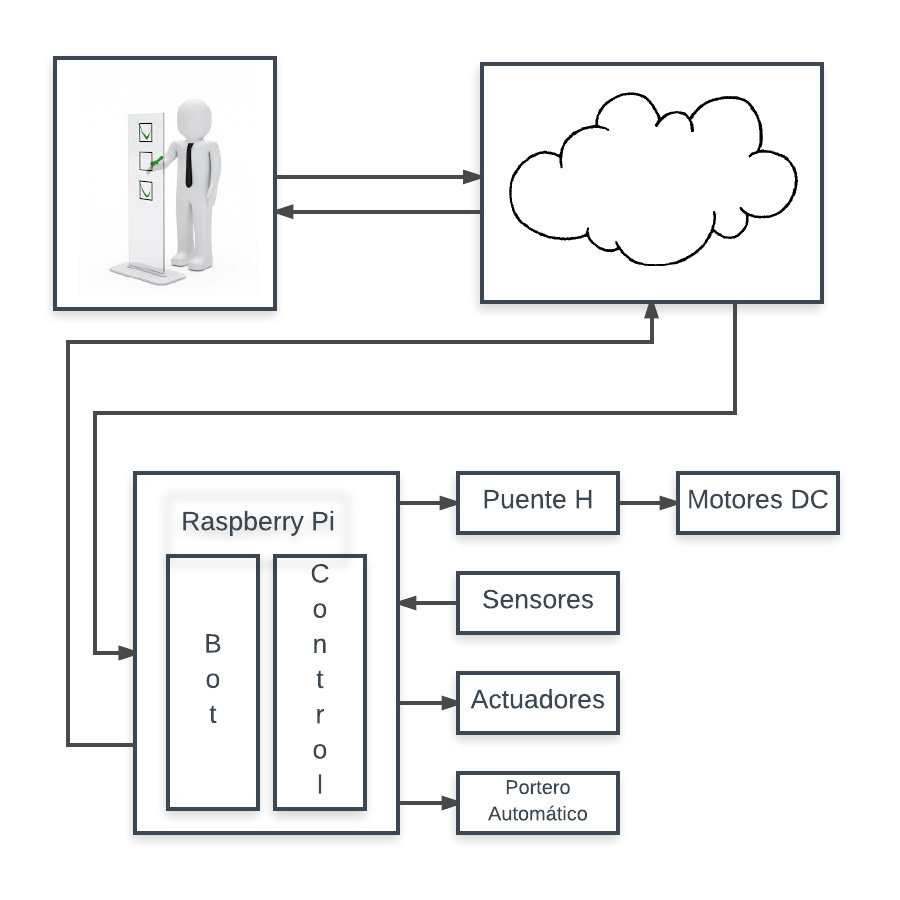
\includegraphics[scale=0.5]{ArqSist}
\caption{Arquitectura del sistema}
\label{fig:arqSist}
\end{figure}

En la figura \ref{fig:arqSist} se muestra la arquitectura del sistema que se va a desarrollar. Como vemos, el usuario no tiene contacto directo con el sistema. Pues aunque se encuentre la Raspberry Pi y el usuario en la misma red, la comunicación se estable con el servidor de telegram de por medio.

Una vez que el usuario envía un comando y el bot lo recibe, éste provoca un evento y envía la orden hacia la lógica de control. La cual actuará en consecuencia de su alrededor.

De igual forma que nosotros enviamos comandos al sistema, el sistema nos devolverá los diferentes datos que recoge por los sensores y servicios que se estén manejando en ese momento.


\section{Desarrollo Software}
Para el desarrollo del software, se va a utilizar NodeJS, para la comunicación con telegram se va a usar un módulo para interactuar con el API oficial de telegram. Este módulo nos proporciona los métodos y eventos principales a la hora de comunicarnos con el bot.

En base a los comandos que el usuario env, se va a desarrollar una máquina de estados que nos permitirá interactuar con nuestro sistema.

Las características que se van a incluir en nuestro sistema domótico son las siguientes:
\begin{itemize}
\item Control de usuarios: el acceso a los comandos de nuestro sistema queda restringido a usuarios autorizados. Se gestionarán dos tipos de permisos, administradores y usuarios.
\item Control de presencia: el sistema domótico mediante el protocolo ARP, puede saber los dispositivos que se encuentran en ese momento en la red. Teniendo en cuenta que según datos estadísticos el 51\% de la población mundial tiene un smartphone. Podemos tener constancia de quien se encuentra en casa y guardar un registro de entrada y salida.
\item Control remoto del portero automático: se dispondrá de una cámara en nuestra puerta la cual nos enviará una foto de quien se encuentra en ella cuando llamen al timbre. Pudiendo también enviar un mensaje de voz mediante Telegram y que este sea reproducido.
\item Control de temperatura: mediante el servicio online \textit{openweathermap}, obtendremos la temperatura en nuestra localización
\item Control de alarma: se desarrollará un sistema de alarma por control remoto, asistido en gran parte por nuestro sistema de control de presencia.
\item Control de sensores y actuadores: con los 18 GPIO de la Raspberry Pi se pueden combinar diferentes sensores y actuadores.
\end{itemize}

\subsection{Máquina de estados}
En la figura \ref{fig:MaqEstPrin} se puede ver el diagrama de flujo de la primera toma de decisiones. 
\begin{figure}[h]
\centering
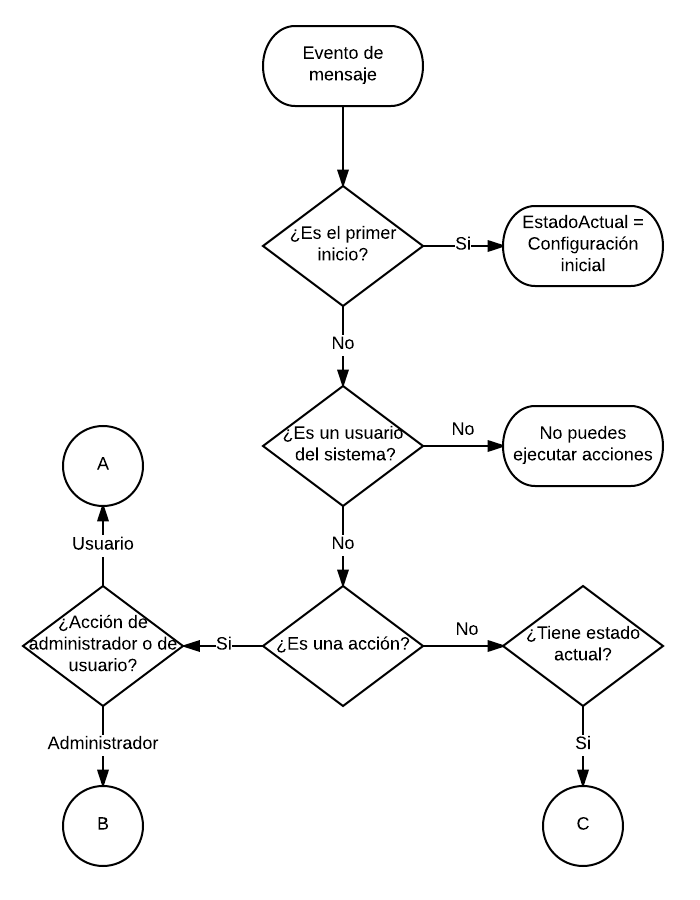
\includegraphics[scale=0.5]{MaqEstPrin}
\caption{Máquina de estados Principal}
\label{fig:MaqEstPrin}
\end{figure}

Cuando nosotros enviamos un mensaje a nuestro control, la primera premisa que tenemos es ser usuario del sistema, si esto no se cumple directamente seremos expulsados.
Si somos usuarios del sistema, se evaluará si hemos enviado una acción o un mensaje, en el caso de ser una acción esta será evaluada como una acción de usuario o de administrador tal y como podemos ver en las figura \ref{fig:MaqEstAcc}, si no coincide con ninguna de ellas se enviará un mensaje de error.

Además de estas acciones, existe una acción especial \textit{/help}, que le muestra al usuario todas las acciones que tiene disponible.

\begin{figure}[h]
\centering
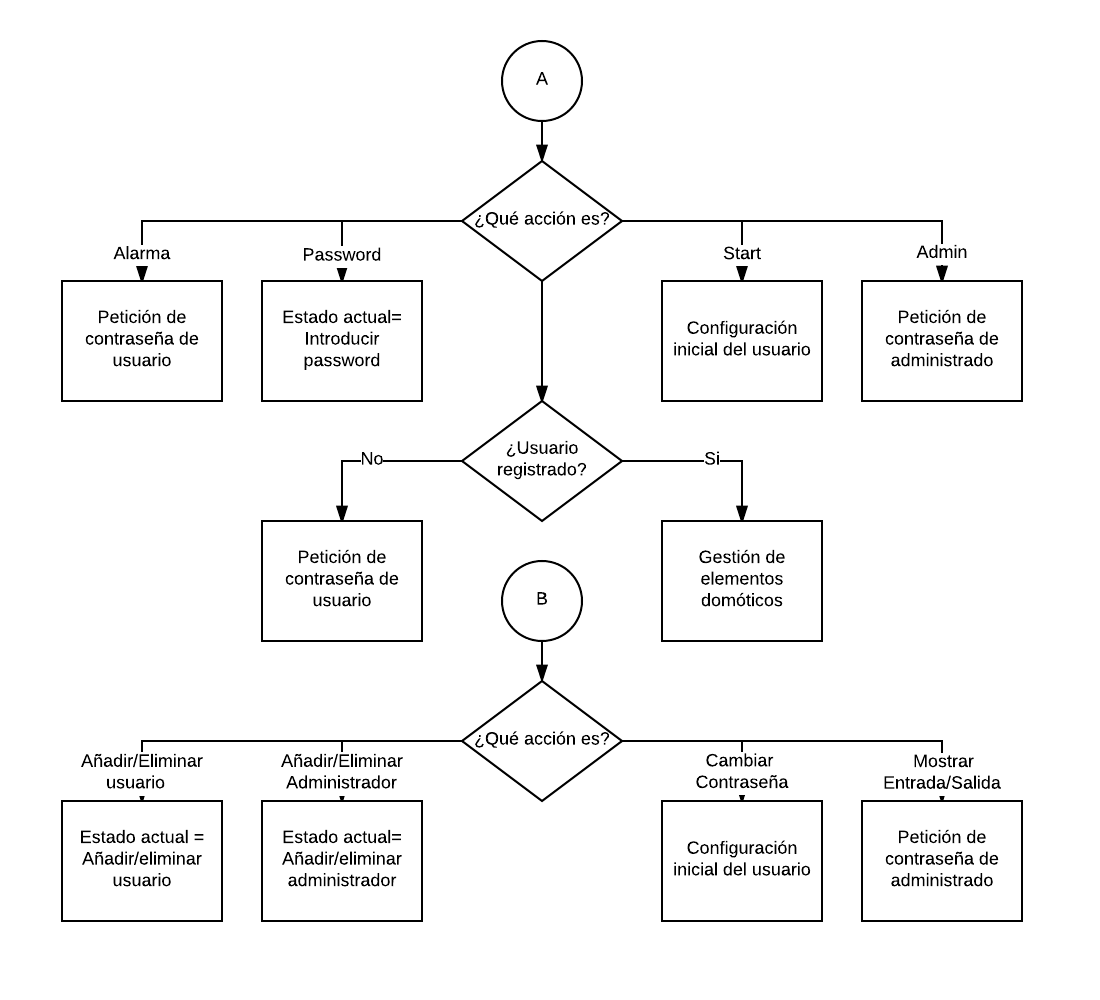
\includegraphics[scale=0.4]{MaqEstAcc}
\caption{Máquina de estados Acciones}
\label{fig:MaqEstAcc}
\end{figure}

En el caso de que no sea una acción, se evaluará si el controlador está esperando una respuesta de nosotros a una acción anterior. Este proceso forma una nueva máquina de estados que estará controlada por la variable \textit{"estado actual"}, que es independiente para cada usuario.
Este tratamiento lo veremos con más detalle en la subsección \ref{sec:ControlUsuarios}

\subsection{Control de usuarios}\label{sec:ControlUsuarios}

En este punto, vamos a ver como se gestionan los diferentes usuarios del sistema y cuales son las posibilidades que tiene cada tipo de usuario.

Cada usuario en telegram se identifica por un ID único que se asigna automáticamente en el momento del registro en la aplicación y además por un alias, también único, el cual se asigna el usuario. Nuestro API puede usar los dos identificadores para enviar los  mensajes, sin embargo, hemos optado por realizar el envío de de los mensajes siempre a través del ID, pues de esta forma tenemos la certeza de que nunca va a fallar el envío del mensaje. 

Los usuarios se almacenan en una variable \textit{users}, identificando a cada usuario por su alias.

\begin{figure}[h]
\centering
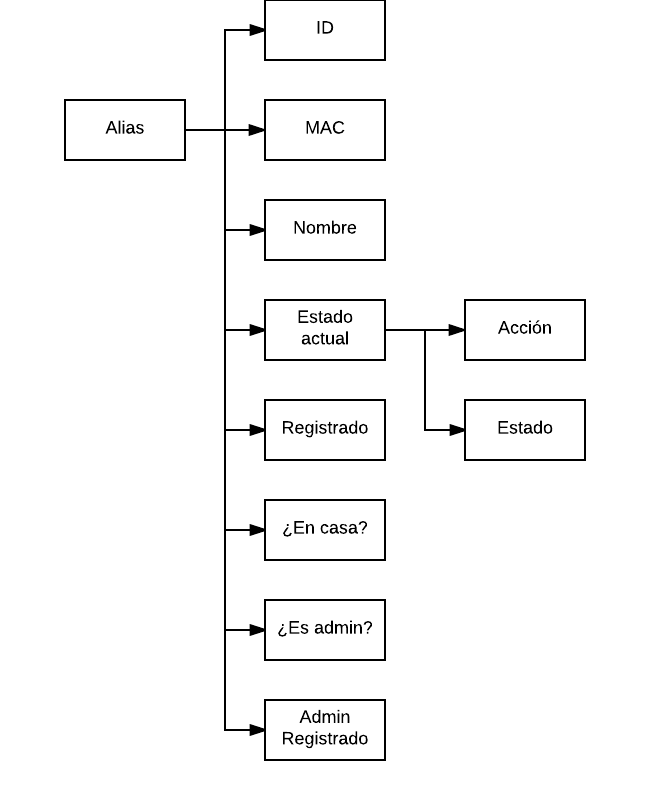
\includegraphics[scale=0.5]{UserEst}
\caption{Estructura de usuario}
\label{fig:UserEst}
\end{figure}

La estructura de  usuario se puede ver en la fig. \ref{fig:UserEst}. A continuación se va a explicar el significado y el uso de cada propiedad:
\begin{itemize}
\item Alias: es el nombre con el que se identificarán a los usuarios. Cuando el bot recibe un mensaje de un usuario, recibimos su alias como identificación.
\item ID: número de identificación, que se usará para enviar mensajes a este usuario cuando sea necesario, al igual que el alias lo recibimos en cada mensaje que envía el usuario.
\item MAC: aquí almacenaremos la MAC del teléfono del usuario. La MAC la se utilizará en el sistema de control de presencia y la obtendremos habilitando un servidor desde nuestra Raspberry Pi y pidiendole al usuario cuando se registre que acceda a ese servidor.
\item Registrado: cuando el usuario introduzca la contraseña de usuario del sistema, en este campo se introducirá la hora del registro, para controlar que cuando se cumpla el tiempo configurado por el administrador este usuario tenga que volver a introducir la contraseña.
\item ¿En casa?: esta propiedad indica si el usuario está en casa. 
\item ¿Es admin?: esta propiedad indica si el usuario es administrador.
\item Admin registrado: tiene la misma función que la propiedad \textit{registrado}, pero esta vez como administrador 
\item Estado actual: esta propiedad nos permite interactuar con el sistema continuamente, cuando se utilice una acción que necesite más información, la propiedad \textit{acción} toma el valor de la acción pedida y la propiedad \textit{estado} se irá actualizando dependiendo de la cantidad de datos que se necesiten.
\end{itemize}

Un apartado importante sobre el control domótico es la seguridad, no se puede permitir que una persona externa se conecte a nuestro sistema. El problema que se encuentra al introducir la contraseña es la imposibilidad de que se edite el mensaje automáticamente por el sistema, ya que telegram sólo ofrece la posibilidad de editar mensajes propios. 

\begin{figure}[h]
\centering
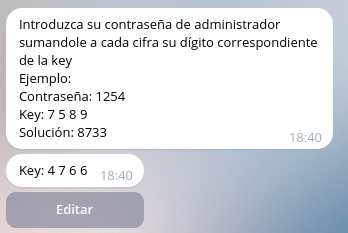
\includegraphics[scale=0.5]{imgPass}
\caption{Proceso introducción contraseña}
\label{fig:imgPass}
\end{figure}

Para subsanar este problema, el sistema generará una key aleatoria, la cual enviará con un botón de edición. El usuario deberá sumar esta key a la contraseña real término a término.
De esta forma, al pulsar el botón de \textit{Editar}, el sistema automáticamente eliminará el mensaje con la key, podemos ver el proceso en la figura \ref{fig:imgPass}

\subsection{Control de presencia}

\subsection{Control remoto del portero automático}

\subsection{Control de temperatura}

\subsection{Control de alarma}

\subsection{Control de sensores y actuadores}

\subsection{Almacenaniento de opciones}
En este apartado, vamos a ver como se almacenan las opciones de forma permanente a la espera para prevenir la pérdida de datos con la caida de la aplicación. La cantidad de información que se maneja no tiene tamaño como para usar una base de datos como mySQL, MongoDB, etc. 
Se ha optado por almacenar los datos persistentes en archivos CSV, de esta forma tenemos implementado un módulo de lectura y escritura de este tipo de archivos para en un futuro poder usar el envío de ficheros CSV para configurar el sistema, añadir usuarios, etc.


\section{Pruebas de Rendimiento}
The conclusion goes here.

\section{Costes}
El tiempo desarrollo de este sistema domótico ha sido de 300 horas, tomando un precio por hora de 30\euro, tenemos un coste de desarrollo de 9000\euro.

Cada sistema tendría un coste fijo que sería la Raspberry, a un precio de 60\euro. Para cubrir los costes con la venta de 100 terminales, cada terminal debería tener un precio de 181.5\euro
(IVA incl.)

A continuación habría que sumar los sensores y actuadores que desea el cliente y el coste de su instalación.

\section{Conclusiones}
The conclusion goes here.

\hfill mds
 
\hfill August 26, 2015

\begin{thebibliography}{1}

\bibitem{IEEEhowto:kopka}
H.~Kopka and P.~W. Daly, \emph{A Guide to {\LaTeX}}, 3rd~ed.\hskip 1em plus
  0.5em minus 0.4em\relax Harlow, England: Addison-Wesley, 1999.

\end{thebibliography}
\end{document}


